\chapter{Problema de Investigación}
\markboth{Problema de Investigación}{Problema de Investigación}

\section{Título}
Desarrollo de solución para integrar la plataforma ``Zendesk Chat''  con el sistema de automatización de conversaciones ``Oracle Digital Assistant''.

\section{Planteamiento del problema}
% cual es el problema? Se necesita automatizar la atencion al cliente via chat pero permites un grado de atención personal de ser necesaria
Zendesk Chat originalmente Zopim, es un producto de software web adquirido por la compañia Zendesk para ofrecer la posibilidad de chat en vivo entre su suite de soluciones en el área de atención al cliente. Debido al éxito que ha tenido Zendesk, el uso de sus productos se ha expandido en el área de soporte, siendo Zendesk Chat la opcion de preferencia para aquellos entes que necesitan ofrecer una forma de interacción directa con sus clientes.

Sin embargo esta solución no es perfecta, entre los defectos podemos nombrar dos que influyen en su implementación por aquellos interesados en el entorno Zendesk. En primer lugar por el volumen de interacciones que pueden generarse en las plataformas en linea, el coste que requeriría un equipo de personal capacitado para la atención al cliente manteniendo un nivel de respuesta a la par de un servicio que busca la interactividad de una plataforma de conversación social es alto, y el segundo punto a considerar como defecto es que una gran parte de las interacciones de soporte de cualquier área son de carácter repetitivo, lo que implica que tareas fácilmente automatizables son llevadas a cabo por personal entrenado sumando un costo extra a la implementación de este producto.

Gracias a que la plataforma Zendesk ofrece interacción vía API para la mayoría de sus productos incluyendo Zendesk Chat, se plantea desarrollar un sistema que conecte Oracle Digital Assistant, la cual es la plataforma de Oracle para la creacion de bots y automatización de interacciones, con Zendesk Chat, ofreciendo así la posibilidad de automatizar interacciones además de permitir a los usuarios de la plataforma Zendesk Chat la opción de habilitar para sus clientes una vía de atención directa en vivo si el sistema automatizado no cumple con sus necesidades.


\section{Justificación}
Los servicios de soporte y atención al cliente son utilizadas como apoyo para un amplio abanico de soluciones. Su uso es esencial para mantener un nivel de calidad y aceptación del producto ante los usuarios del mismo, esto es de especial importancia para plataformas con grandes volúmenes de usuarios, donde la atención se lleva a cabo por medio de aplicaciones similares a plataformas de conversación social, donde el usuario se siente atendido de forma directa. 

La implementación de un sistema automatizado de conversaciones dentro del área de soporte y atención al cliente busca precisamente mejorar el funcionamiento de estas soluciones, al permitir que la atención personalizada se centre en los casos que requieren un nivel de resolución mas complejo, sin sacrificar la sensación de atención personal que aporta una plataforma de conversaciones social.


\section{Objetivo General}

Desarrollar software que permita integrar el sistema de automatización de conversaciones de Oracle Digital Assistant con la plataforma de soporte Zendesk Chat conservando la capacidad de atención al cliente por personal humano.

    
\section{Objetivos Específicos}
    \begin{itemize}
        \item Configurar Oracle Digital Assistant y Zendesk Chat con las herramientas web que ofrecen para permitir integraciones entre aplicaciones de terceros.
        
        \item Implementar un servidor que maneja las solicitudes y respuestas de las plataformas Oracle Digital Assistant y Zendesk Chat.
        
       	\item Desarrollar los algoritmos que traduzcan la estructura de solicitudes y respuestas de los servicios Oracle Digital Assistant a Zendesk Chat y viceversa.
    
    	\item Añadir a la solución desarrollada la capacidad de la operación manual por un agente cuando el usuario lo requiera.
                
        \item Programar la automatización de una conversación en Oracle Digital Assistant para probar el funcionamiento de la integración
        
    \end{itemize}
    
    
    
\section{Solución Propuesta}

Se propone el desarrollo de un servidor que maneje solicitudes de las plataformas Oracle Digital Assistant (ODA) y Zendesk Chat, de tal forma que se logre integrar un sistemas automatizado de conversaciones creado en la plataformas ODA con la plataforma de soporte y atención al cliente Zendesk Chat.

Dicha solución permitirá que tareas repetitivas sean atendidas por el sistema automatizado, manteniendo la interacción con el usuario a travez de la interfaz de chat de la plataforma Zendesk Chat, además se implementara la capacidad para manejar el control del flujo de la conversación entre el sistema automatizado y un agente humano.

    \subsection{Arquitectura conceptual a utilizar}
    Se plantea implementar un servidor web que maneje peticiones de las  plataformas Oracle Digital Assistant y Zendesk Chat, y emita respuestas adecuadas en el formato que dichas plataformas aceptan.
    
    La arquitectura de la solución se puede dividir en dos casos. El primer caso  se distingue por la interacción de ODA con el servidor web, este proceso se demuestra en la figura \ref{fig:arqconoda}, el usuario interactúa con la interfaz de chat administrada por Zendesk Chat, los mensajes del usuario serán transmitidos por Zendesk vía websockets al servidor web, donde serán adaptados para su envió a la plataforma de Oracle. La plataforma de ODA procesara el mensaje y enviara un mensaje de respuesta al servidor web de acuerdo a la configuración del bot, dicho mensaje sera luego transmitido a la plataforma de Zendesk.
    \begin{figure}[htpb]
        \centering
        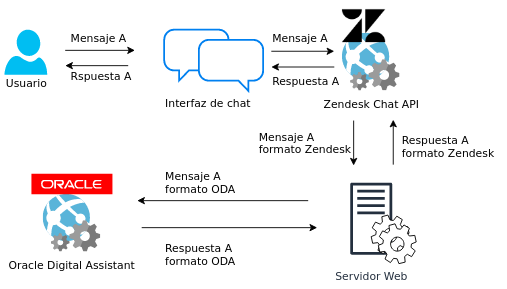
\includegraphics[width=0.85\textwidth]{Figuras/propuestasolucion1.png}
        \caption{Arquitectura conceptual, interacción con ODA}
        \label{fig:arqconoda}
    \end{figure}
    
    En la figura \ref{fig:arqconagente} se presenta el segundo caso; el servidor web recibe una petición de interacción con un agente humano por parte del usuario, el servidor web se encarga de enviar el control de la conversación a Zendesk para que el agente mantenga una conversación directa con el usuario, una vez el agente decida culminar la conversación el servidor web retornara el control al bot.
    
    \begin{figure}[htpb]
        \centering
        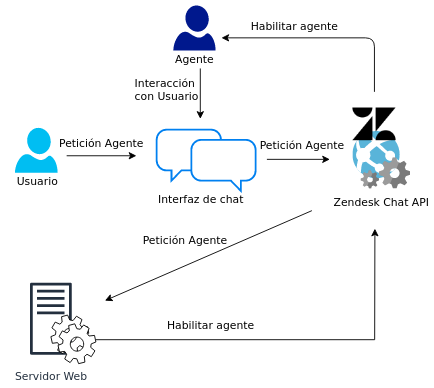
\includegraphics[width=0.85\textwidth]{Figuras/propuestasolucion2.png}
        \caption{Arquitectura conceptual, interacción con Agente}
        \label{fig:arqconagente}
    \end{figure}
    
    
    \subsection{Arquitectura tecnológica a utilizar}
    %Nodejs express librerias oracle zendesk chat
    Para la implementación de la solución se utilizara Node.js para el desarrollo del servidor web y Express.js como el framework principal, esto permitirá hacer uso de las cualidades REST que ofrece Express.js manteniendo un nivel de consistencia y estandarización con la arquitectura REST. Para la interacción con las plataformas de terceros se incluirán las librerías aportadas por Oracle Digital Assistant y Zendesk Chat, estas librerías son desarrolladas en Javascript y están soportadas por Node.js. 
    
    El servidor sera estructurado siguiendo un modelo de microservicios, lo que permitirá un enfoque en la alta mantenibilidad de la solución y facilidad para su implementación y despliegue por un equipo pequeño.
    
    Los datos generados por la aplicación son generados por las plataformas de terceros por lo que la solución no necesita hacer uso de una tecnología de base de datos para su implementación, toda información sera almacenada por Oracle o Zendesk utilizando la tecnología por defectos de sus sistemas.
    
    \subsection{Metodología de desarrollo a utilizar}
    %SCRUM
    %Para guiar el desarrollo de este proyecto se propone el uso de la metodología de desarrollo ágil SCRUM, por su facilidad de adaptación diseñada para ofrecer un valor significativo de forma rápida en todo proyecto. La misma permite presentar soluciones parciales mediante el uso de iteraciones, lo que hará que existan pruebas que contribuyan con el progreso del desarrollo de la aplicación al poder obtener retroalimentación de parte del cliente. 
    
    El desarrollo de este proyecto se llevara bajo un marco metodológico ágil basado en SCRUM, haciendo uso del backlog, los sprint, y la propiedad iterativa del mismo. Sin embargo este proyecto sera llevado por un único individuo por tanto las propiedades del modelo SCRUM aplicadas a equipos no estarán presente como parte de la metodología en este proyecto. 
    
    % \subsection{Descripción del flujo asociado a la solución}
    

\section{Alcance}
    \begin{itemize}
        \item Generar los permisos adecuados en la plataforma Zendesk Chat para integrar por medio de su API REST servicios de terceros.
        
        \item Implementar un servidor en Node.js usando Express.js como framework, instalando en el mismo mediante NPM las librerías ofrecidas por Oracle y Zendesk para el uso con sus productos.
        
        \item Desarrollar un servicio que maneje los mensajes provenientes de Oracle Digital Assistant y traduzca su estructura para ser comprendidos por la plataforma  Zendesk Chat
        
        \item Desarrollo de algoritmo que maneje el uso de mensajes con formatos especiales que incluyan botones o respuestas rápidas entre Zendesk Chat y Oracle Digital Assistant
        
        \item Implementar la capacidad de cambiar el control del flujo de la conversación entre el sistema automatizado y un agente humano.
        
        \item Manejo de errores de conexión y reactivación automática de la conexión por websocket entre Zendesk Chat y el servidor.
        
        \item Configurar un Canal (Channel) de Oracle Digital Assistant, que permita la integración por medio de webhooks y su API REST de aplicaciones de terceros con el servicio ofrecido por Oracle.
                
        \item Crear un sistema de respuestas automáticas usando el producto `Habilidades' (Skills) de Oracle Digital Assistant.
        
        \item Realizar el proceso de integración del sistema de respuestas automatizadas mediante el canal de Oracle Digital Assistant para comprobar el funcionamiento de la integración con Zendesk Chat.
        
        \item Simular el proceso de cambio de control de flujo entre el sistema automatizado y un agente humano en Zendesk Chat.
        
    \end{itemize}